%%
%% This is a LaTeX document formatted using the ACM 'acmlarge' style.
%% It presents a scientific report on User Control in Tourism Recommender Systems.
%%
\documentclass[acmlarge]{acmart}

\AtBeginDocument{%
  \providecommand\BibTeX{{%
    Bib\TeX}}}

\usepackage{graphicx}
\usepackage{float}

%% Rights management information.
\setcopyright{none}
\settopmatter{printacmref=false} % Removes ACM Reference Format
\acmJournal{POMACS}
\acmVolume{1}
\acmNumber{1}
\acmArticle{1}
\acmYear{2026}
\acmMonth{6}
\acmDOI{}

\begin{document}

\title[Empowering Users with Algorithmic Control and Transparency]{Empowering Users with Algorithmic Control and Transparency in Tourism Recommender Systems: A DSA-Compliant Approach}

\author{David Gallob}
\email{david.gallob@tum.de}
\affiliation{%
  \institution{Technical University of Munich}
  \department{School of Computation, Information and Technology}
  \city{Munich}
  \country{Germany}
}

\renewcommand{\shortauthors}{Gallob}

\begin{abstract}
Modern recommender systems that users encounter in daily life are very often "black boxes", which means that users rarely know how their recommendations are generated and they have no control over which items are recommended. In tourism, this leads to a lack of trust and user satisfaction, as users can never be sure if their recommendation is really optimal or influenced by profit maximization goals of the platform. The EU has therefore introduced the Digital Services Act (DSA), a framework which requires platforms to explain their algorithms in an understandable way and offer users a profiling-free alternative. In this paper, a web-based prototype for hotel recommendations which addresses these issues by implementing two algorithms is presented. The web-app offers detailed explanations of the underlying decision algorithms and shows, for each result, how the recommendation was computed. The two algorithms implemented are Weighted Multi-Attribute Utility Theory (MAUT), which lets users set weights on the different attributes (e.g. stars, distance to center, price) on a scale from 0 to 10, and Constraint Filtering, where the user sets hard limits to the attributes (e.g. price must be below 100 Euro per night). This paper details the system architecture as well as the mathematical foundations of the used algorithms along with the UI features explaining the algorithms to the user.
\end{abstract}

\keywords{Recommender Systems, User Control, Multi-Attribute Utility Theory, Constraint Filtering, Digital Services Act, Explainable AI, E-Tourism}

\maketitle

\section{Introduction}
In day-to-day life, recommender systems are ubiquitous, from online shopping and video streaming to hotel and flight recommendation platforms~\cite{adomavicius2005toward}. Many prominent RS do not let users know how their recommendations are generated and offer no direct means of influencing the outcome~\cite{BORRAS20147370}. Those systems are often built on complex algorithms (mainly neural networks) which process enormous amounts of user data to generate suggestions. They rarely explain their underlying logic to users. This lack of transparency can hinder trust and user satisfaction, leading to frustration and cognitive overhead. The tourism domain, where the financial expenditure and emotional investment are generally high, is particularly affected by this issue~\cite{ricci2011travel}.

The Human-Computer Interaction field has focused research on user influence and transparency (explainability) to address these shortcomings~\cite{knijnenburg2012explaining, tintarev2012evaluating}. Instead of using automated profiling, interactive recommender systems give users the ability to influence the recommendation process by adjusting sliders representing attribute weights or setting hard constraints for the attributes (e.g., price or distance).

The demand for transparency is further fueled by the European Union's Digital Services Act, which governs online platforms and aims to protect users' rights. The DSA mandates that online platforms must provide users with transparent information about the main parameters of their recommender systems in an understandable language in plain text and offer options to influence them (Article 27)~\cite{eudsa2022}. Article 38 further obliges very large online platforms (VLOPs) to provide users with at least one option for their recommender systems that is not based on profiling. These articles require developers to shift from black-box profiling towards transparent and user-controlled platforms.

In this paper, the design decisions, architecture, and implementation of a web-application tourism recommender system prototype which is compliant with the DSA are detailed. It addresses the transparency as well as the user influence goals by implementing two algorithms:
\begin{enumerate}
    \item \textbf{Algorithm A: Weighted Multi-Attribute Utility Theory (MAUT)}:
    This algorithm uses sliders to determine weights for hotel attributes (price, location, star rating, customer rating, and public transit access). To prevent user confusion regarding percentages summing up to 100\%, the importance weights are defined on a 0 to 10 scale (where 0 means completely unimportant and 10 is the most important). The algorithm performs a normalization of the attributes and computes a weighted utility score for each hotel. Finally, the hotels are ranked according to their utility score (percentage match).
    \item \textbf{Algorithm B: Constraint-Based Filtering}: 
    In Constraint-Based Filtering, the user defines hard limits for each attribute (e.g., maximum price or minimum rating). All hotels which do not meet the constraints are filtered out. This allows users to specify their preferences in a clear and understandable way without the need for complex mathematical calculations.
\end{enumerate}

The prototype features a dynamic strategy selection landing wizard that ensures that transparency panels are not shown prematurely. Once a strategy is chosen, a dynamic banner is displayed explaining the chosen algorithm in clear words, and offers a button which when pressed shows the mathematical formula of the chosen algorithm for enhanced transparency. The calculated results also offer a collapsible mathematical breakdown (only on user intent to not overwhelm uninterested users) showing a step-by-step calculation of how the result's score was computed. This allows users to understand how the results are generated and how their inputs influence the outcome. The calculation breakdown is generated using KaTeX and renders the exact mathematical formulas and normalization equations used in the calculations, allowing users to trace how their inputs directly translate into the presented results.

\section{Remainder Structure}
The remainder of this paper is structured as follows: In \autoref{sec:related_work}, the related work in current tourism recommender systems, MAUT, and explanation interfaces is presented. \autoref{sec:system_architecture_and_implementation} details the system's architecture and the mock dataset. \autoref{sec:algorithmic_framework} shows the mathematical foundations of the two used algorithms. \autoref{sec:user_interface_design_and_explainability} details the UI design and transparency features. \autoref{sec:future_work} proposes a protocol for a future user study and extensions, and \autoref{sec:conclusion} concludes the paper. In the Appendix, the complete mock database used in the project, followed by the author contribution details and GenAI disclosures are attached.

\section{Related Work}\label{sec:related_work}
Recommender systems' development faces special challenges which are unique to their domain --- such as recommendations for movies and music~\cite{BORRAS20147370}. In the tourism domain, decisions require a lot of rational resources, are infrequent, and have multiple decision attributes. In contrast to low-cost consumer goods, vacation planning involves a high final risk and high emotional expectations, which also leads to a high time commitment. Users therefore take extensive information and comparisons into account and need to express specific constraints before making a final decision~\cite{ricci2011travel}.

Traditional recommender systems  in the tourism domain are mainly divided into three categories~\cite{Sarkar2023, 8308293}:
\begin{itemize}
  \item \textbf{Collaborative filtering:} Builds on historical information of similar users, but suffers from the Cold Start Problem --- New hotels without reviews and seldom travellers without historical ratings lead to wrong recommendations.
  \item \textbf{Content-based:} These systems match item features with the preference profiles of the user. While they get good results, they are often unable to explain their recommendations and to adapt to rapid changes in user needs (e.g., business travelers in central locations versus family budget accommodations).
  \item \textbf{Hybrid:} These recommender systems combine multiple approaches.
\end{itemize}

In order to tackle these limitations, multi-attribute frameworks, i.e., Multi-Attribute Utility Theory (MAUT) for decision making, have been coming to use in interactive recommender systems~\cite{schmitt2002maut}. MAUT is a mathematical algorithm which allows to evaluate alternatives with potentially conflicting attributes~\cite{keeney1993decisions}. The algorithm defines a utility function for every attribute (e.g., mapping location to a utility between 0 and 1) and calculates a weighted sum. MAUT, as shown by Schmitt et al. in 2002~\cite{schmitt2002maut}, is particularly useful in interactive recommender systems, as it takes human decision making processes into account (i.e., user-defined weights). It allows for deficiencies (e.g., high price) to be evened out by a high value in another attribute (e.g., excellent location).

Constraint-based recommender systems are non-compensatory in contrast. They do not calculate a score, but filter out items violating user-defined limits based on explicit knowledge about the items~\cite{ricci2011travel}. This approach is easy to understand and does not require user profiling, perfectly aligning with the EU's DSA~\cite{eudsa2022}.

Earlier research has shown that the success of interactive recommender systems strongly relies on their UIs~\cite{mcnee2006being,swearingen2001beyond}. Therefore, providing explanations in the UI improves user understanding as well as their trust and perceived control over the system~\cite{tintarev2012evaluating}. Knijnenburg et al.~\cite{knijnenburg2012explaining} showed that their proposed framework offering user control paired with high explainability results in higher user satisfaction and acceptance. The integration of sliders for defining weights and mathematical breakdowns along with transparency panels investigated in this paper builds on those findings to build an explainable and transparent UI for user satisfaction and to meet the DSA requirements.

\section{System Architecture and Implementation}\label{sec:system_architecture_and_implementation}
The prototype is designed as a web application. The technical architecture consists of React, Vite for the build system, and vanilla CSS for layout and styling. Client-side math rendering is powered by KaTeX, a fast LaTeX math rendering library, integrated via a custom React wrapper. The system architecture is structured to support real-time user interaction.

The application state manages:
\begin{itemize}
  \item The selected city (Munich vs. Vienna).
  \item The selected algorithm (MAUT vs. Constraint-based).
  \item The five attribute weights ($w_i \in [0, 10]$) for the MAUT mode.
  \item The five attribute limits for the Constraint Filtering mode.
  \item The global formula toggle (including a switch for the explanation board, showing the matching explanations).
\end{itemize}

In the dataset, which is stored in a static module ``data.js'', 20 hotels (10 for each city) are stored. The hotels represent a realistic and diverse range of accommodations, which range from low-budget hostels to luxury five-star hotels. Each hotel is uniquely defined by an identifier, name, city description, and five attributes:
\begin{enumerate}
  \item \textbf{Price per Night}: Ranging from \$35 (Hostel Vienna West) to \$550 (Mandarin Oriental Munich).
  \item \textbf{Distance to Center}: Distance from the historical city center (Stephansplatz in Vienna, Marienplatz in Munich). Ranging from 0.1 km (Stephansplatz) to 28.0 km (Airport Express Inn Munich).
  \item \textbf{Star Rating}: Ranging from 1 (basic tourist class) to 5 stars (luxury class).
  \item \textbf{Guest Review Score}: A continuous rating between 1.0 (worst) and 10.0 (excellent), representing aggregated guest satisfaction.
  \item \textbf{Public Transport Access Score}: A rating between 1.0 (poor) and 10.0 (excellent), representing proximity to subway stations, tram lines, and frequency of transit services.
\end{enumerate}
The application calculates and updates the recommendations in real-time if a user modifies the slider weights or switches the algorithm. This renders a ``calculate'' button useless, improving user-friendliness. This is possible as the calculations on the fixed dataset are performed client-side.

\section{Algorithmic Framework}\label{sec:algorithmic_framework}
To support the user-controlled interaction model, this section expains the mathematical models behind the algorithms in the recommendation engine.

\subsection{Algorithm A: Weighted Multi-Attribute Utility Theory (MAUT)}
This algorithm evaluates each hotel in the chosen city by mapping the hotels attribute values to normalized utility scores and computing a weighted average. The process is performed in three steps:

\subsubsection{Normalization of Attributes}
As the attributes use incomparable units (e.g., USD, kilometers, stars), they must first be normalized to a standard scale $u(v) \in [0, 1]$, where $0$ represents the worst possible utility and $1$ represents the best possible utility.

The hotel attributes are split into cost metrics (where lower values are better, like price and distance) and benefit metrics (where higher values are better, like star ratings, guest review scores, and public transport access). The prototype implements two normalization strategies:

\textbf{Relative Normalization}: Used for cost metrics, as these values do not have clear upper and lower bounds. Therefore the items are compared to each other to define the thresholds. The normalized utility score $u(v)$ for an attribute value $v$ of an item is calculated as:
\begin{equation}\label{eq:norm_relative}
  u(v) = \frac{v_{\max} - v}{v_{\max} - v_{\min}}
\end{equation}
where:
\begin{itemize}
  \item $v$ is the value of the hotel
  \item $v_{\min}$ and $v_{\max}$ are the minimum/maximum value of this attribute of all hotels in the selected city.
\end{itemize}


\textbf{Absolute Normalization}: This is used for benefit attributes (stars, rating, and public transport access) because these values have clear intrinsic values for the best and worst option (e.g. stars, guest review rating). In addition, normalizing these scores relatively could artificially exaggerate small differences (e.g. ranking a hotel with 8.5 rating as 0 utility if it is the lowest in the city).
For stars (on a 1 to 5 scale), the utility is calculated as following:
\begin{equation}\label{eq:norm_stars}
  u_{\text{stars}}(v) = \frac{v - 1}{4}
\end{equation}
where $v$ is the amount of stars of the hotel (from 1 to 5).

For the guest review rating scores and the public transport access score (both ranging on a 1 to 10 scale), the utility is calculated as following:
\begin{equation}\label{eq:norm_rating_transit}
  u_{\text{rating/transport}}(v) = \frac{v - 1}{9}
\end{equation}
where $v$ is the guest review score or public transport access score of the hotel (from 1 to 10).

\subsubsection{Weighted Aggregation}
After the initial normalized attribute scores are calculated, the utility scores are weighted and summed up. Let $w_i$ be the user given weight to the attribute $i$ (where $w_i \in [0, 10]$), and $u_i$ be the prior calculated normalized utility score of the attribute $i$ for the hotel item. The total utility $U$ is calculated as:
\begin{equation}\label{eq:maut}
  U = \frac{\sum_{i=1}^{5} w_i \cdot u_i}{\sum_{i=1}^{5} w_i} \times 100\%
\end{equation}
The calculated hotels are sorted and shown to the user in descending order.

\subsection{Algorithm B: Constraint-Based Filtering}
The Constraint-Based Filtering algorithm does not calculate a mathematical match score or rank the hotels. Instead, it checks if the set of hotels in the selected city comply to user set constraints. A hotel is in the result set (i.e. shown to the user) if and only if it satisfies the logical conjunction:
\begin{equation}\label{eq:filtering}
  \text{Price} \le P_{\max} \ \land \ \text{Distance} \le D_{\max} \ \land \ \text{Stars} \ge S_{\min} \ \land \ \text{Rating} \ge R_{\min} \ \land \ \text{Transport} \ge T_{\min}
\end{equation}
where:
\begin{itemize}
  \item $P_{\max}$ is the maximum price threshold defined by the user.
  \item $D_{\max}$ is the maximum distance threshold defined by the user.
  \item $S_{\min}, R_{\min}, T_{\min}$ are the minimum stars, guest review rating, and public transport access scores thresholds defined by the user.
\end{itemize}
This filtering logic is non-compensatory --- hotels are not compared to each other and relatively ranked. All hotels are simultaneously checked and excluded form the results if a single constraint is violated.

\subsection{Comparison of Decision Logic}
The two models are fundamentally different in their decision-making styles: The biggest difference is that MAUT will (due to its ranking nature) show results to the user that are completely irrelevant to the user, as it is more a sorting approach than a filtering approach. Constraint-filtering on the other hand does not show the aforementioned uninteresting results, but delivers a result set to the user, without giving information of how well an item fit the user's limits. The differences are summarized in Table~\ref{tab:comparison}.

\begin{table}[h]
  \caption{Comparison of the Implemented Algorithmic Paradigms}
  \label{tab:comparison}
  \begin{tabular}{lll}
    \toprule
    Dimension & Algorithm A: Weighted MAUT & Algorithm B: Constraint Filtering \\
    \midrule
    \textbf{Decision Logic} & Compensatory (trade-offs allowed) & Non-compensatory (hard boundaries) \\
    \textbf{Output Type} & Ranked list with continuous match scores & Unordered subset of matching items \\
    \textbf{User Controls} & Relative importance weights ($w_i \in [0, 10]$) & Threshold limits ($P_{\text{max}}, D_{\text{max}}$, etc.) \\
    \textbf{Cognitive Style} & Optimizing & Screening / Satisficing \\
    \textbf{DSA Compliance} & Explains weights & Explains inclusion/exclusion criteria \\
    \textbf{Profiling Dependency} & None (Profiling-free, real-time input) & None (Profiling-free, real-time input) \\
    \bottomrule
  \end{tabular}
\end{table}

\subsection{Quality Assurance and Algorithmic Verification}
In order to ensure that the prototype is stable and mathematically correct, the code of the algorithm was built in a standalone module (\texttt{src/recommenderEngine.js}). There, for the verification a unit testing suite was appended (\texttt{run-tests.js}) consisting of exactly 60 different test cases (30 for Weighted MAUT and 30 for Constraint-Based Filtering) for edge cases and different input parameters patterns.

\subsubsection{MAUT Logic Verification (30 Cases)}
The 30 MAUT test cases evaluate the logic of normalization and scoring:
\begin{itemize}
  \item \textbf{Weight Boundary Conditions (5 cases)}: These tests verify that equal weights result in equal ranking results, zero weights do not result in division by zero and that no negative weights and no positive weights above 10 are possible.
  \item \textbf{Price relative cost normalization (5 cases)}: Confirms that the Relative Normalization works as expected: correct mapping of the lowest price to utility 1, highest price to utility 0, and values in between are correctly mapped proportionally. Additionally, it is also verified that no division by zero occurs when all items have the same price (algorithm could map them all to 0 as they all are the ``worst'' option). These tests are run for all other attributes:
  \item \textbf{Distance relative cost normalization (5 cases)}: Verifies that the closest hotel maps to the utility of 1.0, furthest hotel to the utility 0.0, and out-of-bound distances are clamped.
  \item \textbf{Absolute Normalizations (5 cases)}: Asserts that the absolute utility mappings for stars (1-to-5 scale) and guest ratings/public transport scores (1-to-10 scale) are correct.
  \item \textbf{Weight Dominance and Flipped Rankings (5 cases)}: These tests test that highly weighted attributes dominate the ranking and changing weights correctly changes the ranking order as expected.
  \item \textbf{Robustness and Sorting (5 cases)}: Verifies the edge cases for empty list inputs, null inputs, missing weight keys, strict descending sorting order of match scores, and correct formatting of breakdown scores.
\end{itemize}

\subsubsection{Constraint-Based Filtering Verification (30 Cases)}
The 30 filtering test cases check the correctness of the logical conjunction:
\begin{itemize}
  \item \textbf{Individual Attribute Constraints (25 cases)}: 
  These test check the price, location, amount of stars, guest review scores, and public transit access scores separately. For each category, there are 5 tests that verify exclusions and inclusions and that constraints may result in empty sets and in sets with all items included. Also, it is checked that null values lead to the usage of fallback values.
\end{itemize}
All test cases run with its own mock database and pass.

\section{User Interface Design and Explainability}\label{sec:user_interface_design_and_explainability}
The prototype frontend interface was developed with the help of Gemini 3.5\footnote{\url{https://deepmind.google/models/gemini/flash/}} in a modern style with smooth animations to create a premium and modern UI. The UI was also designed to feature maximal explainability for the users. 

\subsection{Interactive Wizard for Algorithm Selection}
Prior iterations showed detailed algorithm explanations before the selection, leading to overloading new users (see the previous cluttered layout in Figure~\ref{fig:old_board}). This issue was tackled by implementing a landing page which explains the available algorithms in simple words and prompts the user to select an algorithm. The user is shown 2 cards to select from:
\begin{itemize}
  \item \textbf{Weighted MAUT Card}: Focuses on compensatory trade-offs. It explains that the user can rate attributes on a scale of 0 to 10, resulting in a ranked list of hotels with percentage match scores.
  \item \textbf{Constraint-Guided Card}: Focuses on strict non-compensatory boundaries. It explains that the user can set threshold limits to eliminate hotels violating any criteria.
\end{itemize}
Afterwards, the user may set the weights or constraints depending on their chosen algorithm and is shown a transparency board, which details the algorithm. This landing-page approach makes the prototype more transparent, as it explains the logic to all users in the beginning. The user may always return to the screen and change their choice by clicking on a ``Switch Algorithm'' button or change the algorithm directly via a switch on the main page.

\begin{figure}[htbp]
  \centering
  \Description{Dashboard view of the previous cluttered user interface design, which loaded all information panels simultaneously and caused cognitive overload.}
  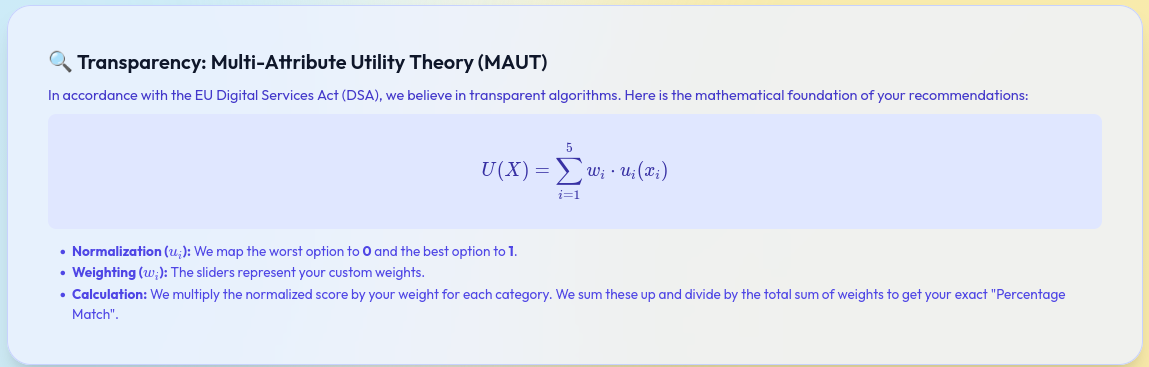
\includegraphics[width=0.6\textwidth]{../presentation_latex/screens/OldOverloadedBoard.png}
  \caption{Previous cluttered transparency board design that led to premature disclosure of complex information.}
  \label{fig:old_board}
\end{figure}

\subsection{DSA-Compliant Explanation Interfaces}
To comply with the requirements of the Digital Services Act, transparency mechanisms are built directly into the primary interaction flow rather than being hidden in auxiliary pages.

\subsubsection{Global Explanation Banners}
At the top of the interface, a dedicated, colored information card dynamically adapts to the selected algorithm.
\begin{itemize}
  \item In \textbf{Weighted MAUT} mode, the banner displays a blue theme, introducing the concept of multi-attribute weighting (see Figure~\ref{fig:maut_interface}).
  \item In \textbf{Constraint-Guided} mode, the banner displays a green theme, introducing the logic of set reduction and non-compensatory filtering (see Figure~\ref{fig:constraint_interface}).
\end{itemize}

Both banners include a "Show Mathematical Details" toggle button. Clicking this button expands a sub-panel that renders the mathematical equations in LaTeX (Equation~\ref{eq:maut} for MAUT, and Equation~\ref{eq:filtering} for Constraint-Guided Filtering) alongside a list of definitions. This design provides a tiered explanation model: novice users receive a brief, plain-language summary of how the parameters are aggregated, while expert users or regulators can inspect the exact mathematical formulas.

\begin{figure}[htbp]
  \centering
  \Description{Left panel shows the five horizontal importance weight sliders with 0 to 10 scale bounds. Right panel shows the corresponding blue Weighted MAUT algorithm explanation card.}
  \begin{minipage}{0.48\textwidth}
    \centering
    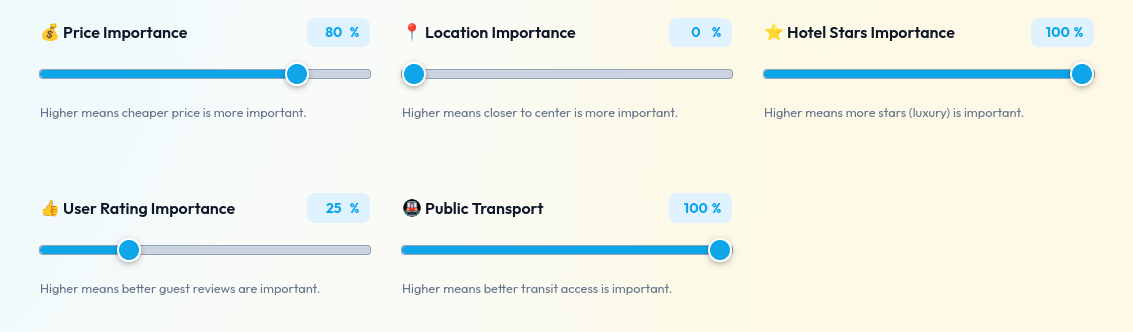
\includegraphics[width=\textwidth]{../presentation_latex/screens/Sliders.png}
  \end{minipage}
  \hfill
  \begin{minipage}{0.48\textwidth}
    \centering
    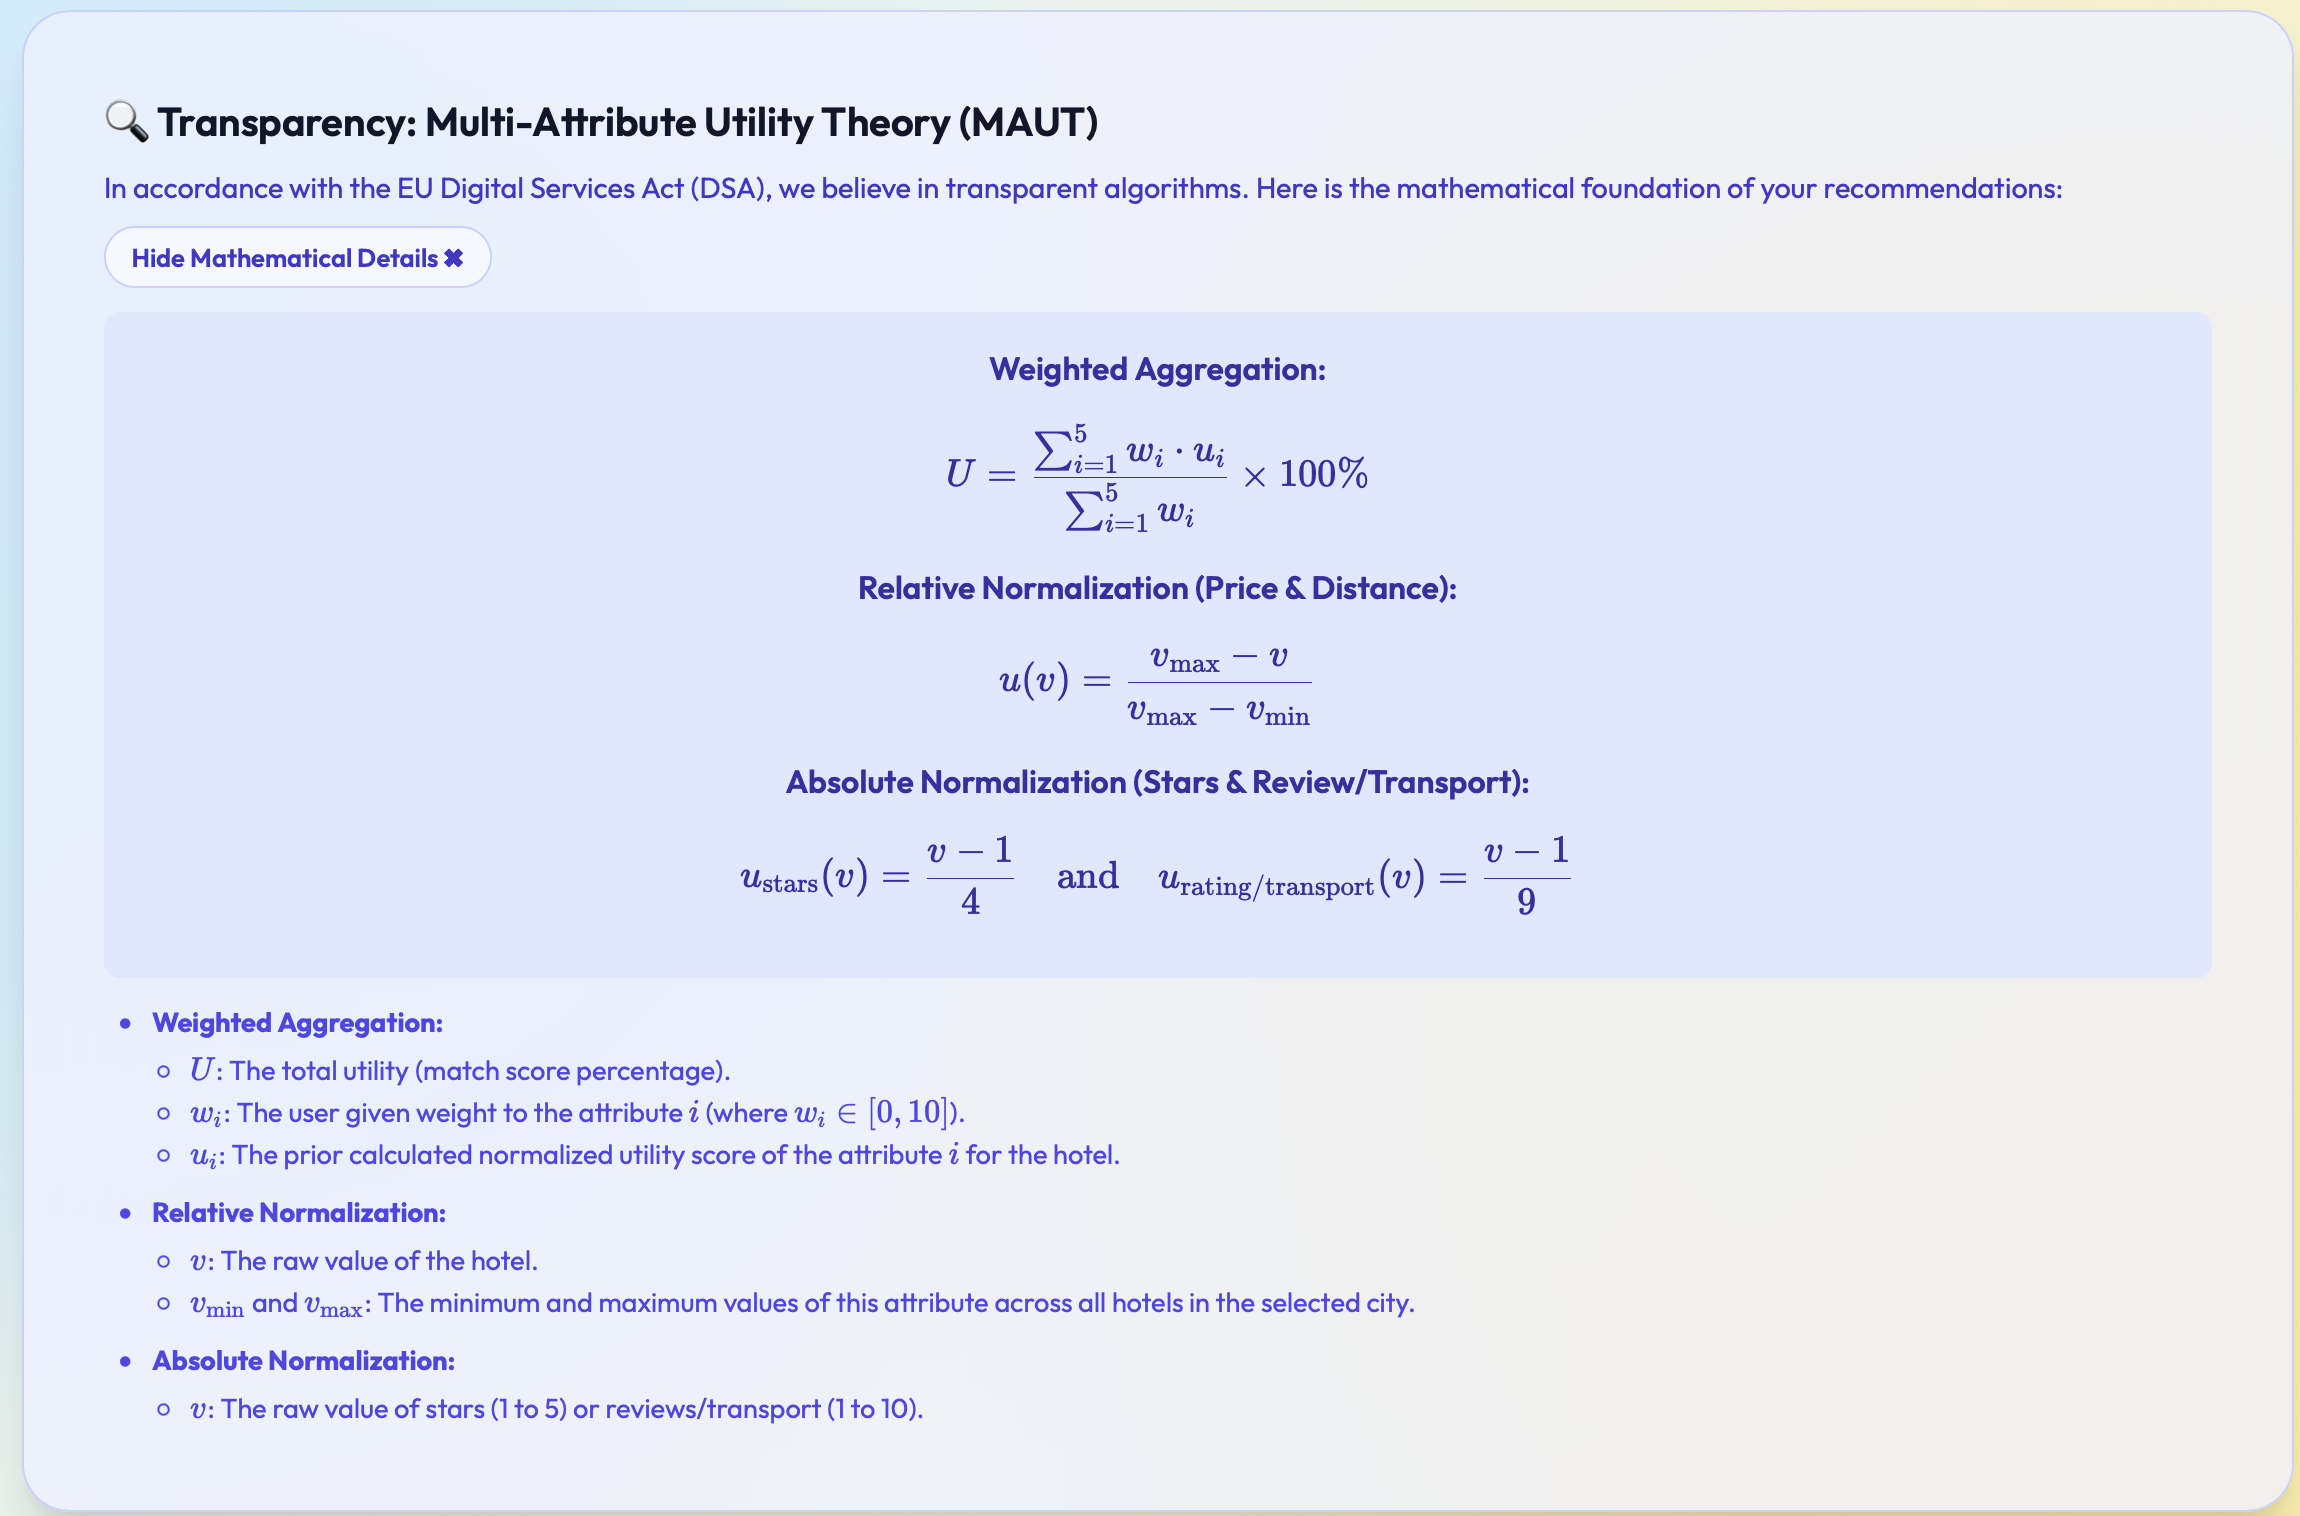
\includegraphics[width=\textwidth]{../presentation_latex/screens/newmaut.png}
  \end{minipage}
  \caption{Weighted MAUT user controls (left) and the dynamic blue explanation banner showing algorithmic details (right).}
  \label{fig:maut_interface}
\end{figure}

\begin{figure}[htbp]
  \centering
  \Description{Constraint-based filtering interface showing threshold range sliders for price, distance, stars, rating, and public transit, alongside the green algorithm explanation banner.}
  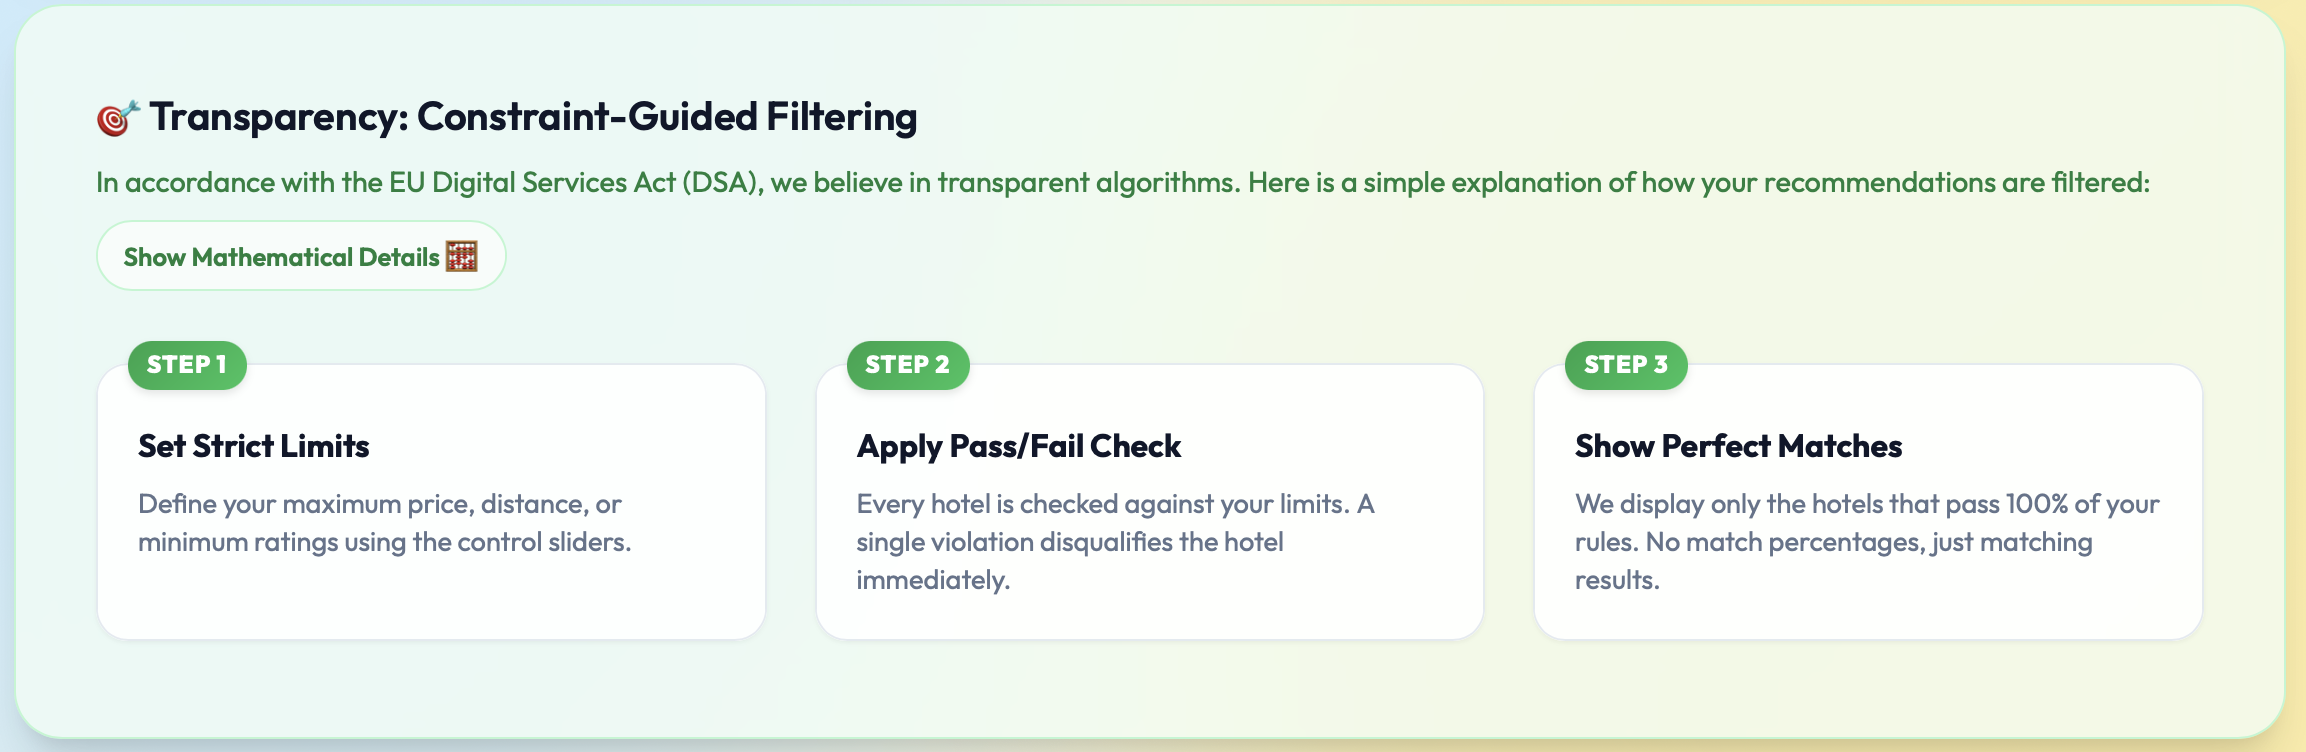
\includegraphics[width=0.7\textwidth]{../presentation_latex/screens/Constraint.png}
  \caption{Constraint-based filtering interface featuring threshold sliders and the dynamic green explanation banner.}
  \label{fig:constraint_interface}
\end{figure}

\subsubsection{On-Demand Collapsible Math Breakdowns}
For the Weighted MAUT mode, each hotel card features a "Show Mathematical Breakdown" button. Expanding this panel reveals a step-by-step trace of the utility calculation for that specific hotel (see Figure~\ref{fig:math_breakdown}).
The panel displays:
\begin{itemize}
  \item The general formula.
  \item A tabular breakdown for each of the five attributes, displaying the normalized utility score, the user-defined weight, and the product.
  \item The summation step, showing the sum of products divided by the sum of weights.
  \item The final rounded match percentage.
\end{itemize}

This feature provides absolute transparency, eliminating the perception of the recommender system as a black box. The user can see exactly why a hotel is ranked first or second, and can directly trace the mathematical impact of adjusting a slider.

\begin{figure}[htbp]
  \centering
  \Description{Collapsible table showing attribute values, normalized utilities, user weight values, multiplication products, and the final sum normalization to calculate the percentage match score.}
  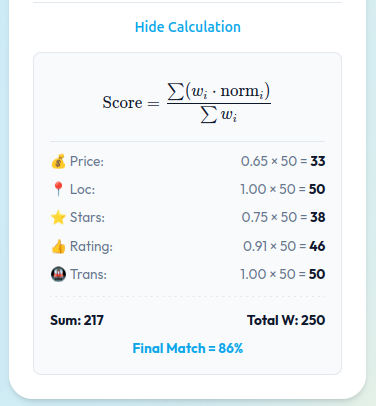
\includegraphics[width=0.3\textwidth]{../presentation_latex/screens/Calculations.png}
  \caption{Collapsible step-by-step mathematical breakdown showing the exact utility calculations for a hotel.}
  \label{fig:math_breakdown}
\end{figure}

\section{Future Work}\label{sec:future_work}
While the current prototype demonstrates the feasibility of user-controlled, transparent tourism recommenders, several research and development paths remain open.

\subsection{The Hybrid Algorithmic Approach}
A natural evolution of the two modes is a hybrid algorithm that combines the strengths of both. Currently:
\begin{itemize}
  \item Weighted MAUT is compensatory, which can lead to high cognitive load as users must constantly balance multiple sliders to filter out unacceptable options.
  \item Constraint-Based Filtering is non-compensatory and does not rank the matching items, which can leave the user with too many options or an empty set.
\end{itemize}
A hybrid recommender would operate as a two-stage pipeline:
\begin{enumerate}
  \item \textbf{Stage 1: Constraint Filtering (Non-Compensatory screening)}: The system applies user-defined constraints to filter out hotels that are completely unacceptable (e.g., price $> \$250$, or distance $> 10$ km). This reduces the candidate pool to a set of feasible options.
  \item \textbf{Stage 2: Weighted MAUT (Compensatory ranking)}: The system applies the user's preference weights to rank only the hotels that passed Stage 1.
\end{enumerate}
This hybrid approach represents a realistic model of human decision-making, where decision-makers first eliminate unacceptable alternatives and then optimize among the survivors. It maintains full transparency and complies with the DSA, while reducing user cognitive load.

\subsection{Proposed User Evaluation Protocol}
To evaluate the user experience (UX) and the effectiveness of the explainability features, a controlled user study protocol is proposed.

\subsubsection{Hypotheses}
Three primary hypotheses are formulated:
\begin{itemize}
  \item \textbf{H1 (Perceived Control)}: Users interacting with the Weighted MAUT or Constraint Filtering interfaces report a higher sense of control over recommendations compared to a baseline "black-box" interface.
  \item \textbf{H2 (System Trust)}: Exposing the collapsible mathematical breakdown panels increases user trust in the system's recommendations without causing information overload.
  \item \textbf{H3 (DSA Compliance Impact)}: The presence of the global explanation banner and KaTeX formulas increases user comprehension of the algorithm's inner workings.
\end{itemize}

\subsubsection{Experimental Design}
A within-subjects laboratory study with $N=30$ participants is proposed. Each participant will perform travel planning tasks under three experimental conditions:
\begin{enumerate}
    \item \textbf{Condition 1 (Baseline - Black Box)}: A traditional recommender interface displaying hotel cards ranked by a hidden algorithm, with no sliders and no explanation panels.
    \item \textbf{Condition 2 (Weighted MAUT with On-Demand Explanations)}: The interactive slider-based interface with collapsible math breakdown panels.
    \item \textbf{Condition 3 (Constraint Filtering with Explanations)}: The constraint-based interface showing absolute threshold sliders.
\end{enumerate}

The ordering of conditions will be counterbalanced to prevent learning effects. Following each condition, participants will complete standardized questionnaires to measure:
\begin{itemize}
  \item \textbf{System Usability}: Measured via the System Usability Scale (SUS).
  \item \textbf{User Experience \& Trust}: Measured using the ResQue (Recommender Systems Quality of Experience) framework, focusing on trust, perceived accuracy, control, and transparency.
  \item \textbf{Cognitive Load}: Measured via the NASA-TLX (Task Load Index) to evaluate if exposing mathematical details increases mental demand.
\end{itemize}
The results of this study will guide the refinement of the UI, helping to strike a balance between complete mathematical transparency and user cognitive ease.

\section{Conclusion}\label{sec:conclusion}
The era of black-box recommender systems is facing both user-experience and regulatory challenges. This paper presented an interactive, transparent tourism recommender system prototype designed to address the compliance requirements of the EU Digital Services Act (DSA). By implementing both a compensatory Weighted Multi-Attribute Utility Theory (MAUT) model and a non-compensatory Constraint-Based Filtering model, the prototype provides users with direct, profiling-free control over recommendation logic. The weights are configured on an intuitive 0 to 10 scale to prevent percentage-summing confusion. We integrated tiered explainability features, combining simple plain-language summaries with on-demand, KaTeX-rendered mathematical breakdowns. Finally, we analyzed and resolved mathematical edge cases, including division-by-zero singularities and score overshooting, ensuring a stable and robust system. This architecture serves as a blueprint for developers seeking to combine rich user control, modern web aesthetics, and strict regulatory compliance in recommender system design.

\begin{acks}
The author would like to thank the teaching staff of the Lab Course: Projects in Recommender Systems (SS 2026) at the Chair of Connected Mobility, Technical University of Munich, for their guidance and feedback throughout the project.
\end{acks}

\bibliographystyle{ACM-Reference-Format}
\bibliography{sample-base}

\appendix

\section{Complete Hotel Database}
Table~\ref{tab:database} presents the complete dataset of 20 hotels used in the recommender system prototype, split between Vienna (v1--v10) and Munich (m1--m10).

\begin{table}[h]
  \caption{Hotel Database Attributes}
  \label{tab:database}
  \begin{tabular}{llrrrrl}
    \toprule
    ID & Hotel Name & Price (\$/night) & Distance (km) & Stars & Rating (/10) & Transport (/10) \\
    \midrule
    \multicolumn{7}{c}{\textbf{Vienna Hotels}} \\
    \midrule
    v1 & Grand Imperial Vienna & 350 & 0.5 & 5 & 9.6 & 9.5 \\
    v2 & Boutique Hotel am Stephansplatz & 180 & 0.1 & 4 & 9.2 & 10.0 \\
    v3 & Danube Riverside Hotel & 95 & 4.5 & 3 & 8.0 & 6.5 \\
    v4 & Schönbrunn Palace Suites & 290 & 6.0 & 5 & 9.8 & 8.0 \\
    v5 & Hostel Vienna West & 35 & 3.2 & 1 & 7.5 & 9.0 \\
    v6 & Art Deco Hotel Prater & 140 & 2.8 & 4 & 8.7 & 8.5 \\
    v7 & Economy Inn Vienna & 60 & 5.5 & 2 & 6.8 & 5.0 \\
    v8 & Museum Quarter Retreat & 210 & 1.2 & 4 & 9.4 & 9.0 \\
    v9 & Green Oasis Hotel & 110 & 7.5 & 3 & 8.9 & 4.0 \\
    v10 & The Ritz-Carlton Vienna & 450 & 0.8 & 5 & 9.7 & 10.0 \\
    \midrule
    \multicolumn{7}{c}{\textbf{Munich Hotels}} \\
    \midrule
    m1 & Bayerischer Hof & 420 & 0.4 & 5 & 9.5 & 9.5 \\
    m2 & Marienplatz Business Hotel & 160 & 0.2 & 4 & 8.8 & 10.0 \\
    m3 & Oktoberfest Lodge & 85 & 2.5 & 2 & 7.2 & 8.0 \\
    m4 & Englischer Garten Retreat & 250 & 3.0 & 4 & 9.3 & 7.0 \\
    m5 & Schwabing Youth Hostel & 40 & 4.0 & 1 & 8.1 & 8.5 \\
    m6 & Olympic Park Hotel & 130 & 6.5 & 3 & 8.5 & 7.5 \\
    m7 & Airport Express Inn & 90 & 28.0 & 3 & 7.8 & 9.0 \\
    m8 & Viktualienmarkt Boutique & 190 & 0.6 & 4 & 9.1 & 9.5 \\
    m9 & Isar River View & 210 & 1.8 & 4 & 8.9 & 6.0 \\
    m10 & Mandarin Oriental Munich & 550 & 0.5 & 5 & 9.8 & 9.5 \\
    \bottomrule
  \end{tabular}
\end{table}

\section{Author Information and Contribution Details}
As a single-author project, Table~\ref{tab:contributions} summarizes the details and contributions of the student.

\begin{table}[h]
  \caption{Project Contributor Details}
  \label{tab:contributions}
  \begin{tabular}{lllp{7cm}}
    \toprule
    Name & Email & GitHub Handle & Contributions \\
    \midrule
    David Gallob & david.gallob@tum.de & davidgallob & Conceptualized and implemented the entire project, including the React web application, MAUT/filtering algorithms, explainability features, user study protocol, and final documentation. \\
    \bottomrule
  \end{tabular}
\end{table}

\section{Generative AI Disclosure}
This project utilized Generative AI tools (specifically Google DeepMind's Gemini 3.5 Flash) during development. The AI was employed as a pair-programming assistant to:
\begin{itemize}
  \item Draft and optimize the user interface layouts and CSS styling rules.
  \item Debug and recommend JavaScript state handling best practices.
  \item Assist in structuring, polishing, and editing the LaTeX code of this scientific report.
\end{itemize}
All design decisions, algorithmic formulations, bug resolutions, and report text were audited, verified, and approved by the human author to ensure compliance with the scientific standards of the Technical University of Munich.
\end{document}
\endinput
